\hypertarget{part-2-treemap-2}{%
\section{Part 2, Treemap 2}\label{part-2-treemap-2}}

\centering
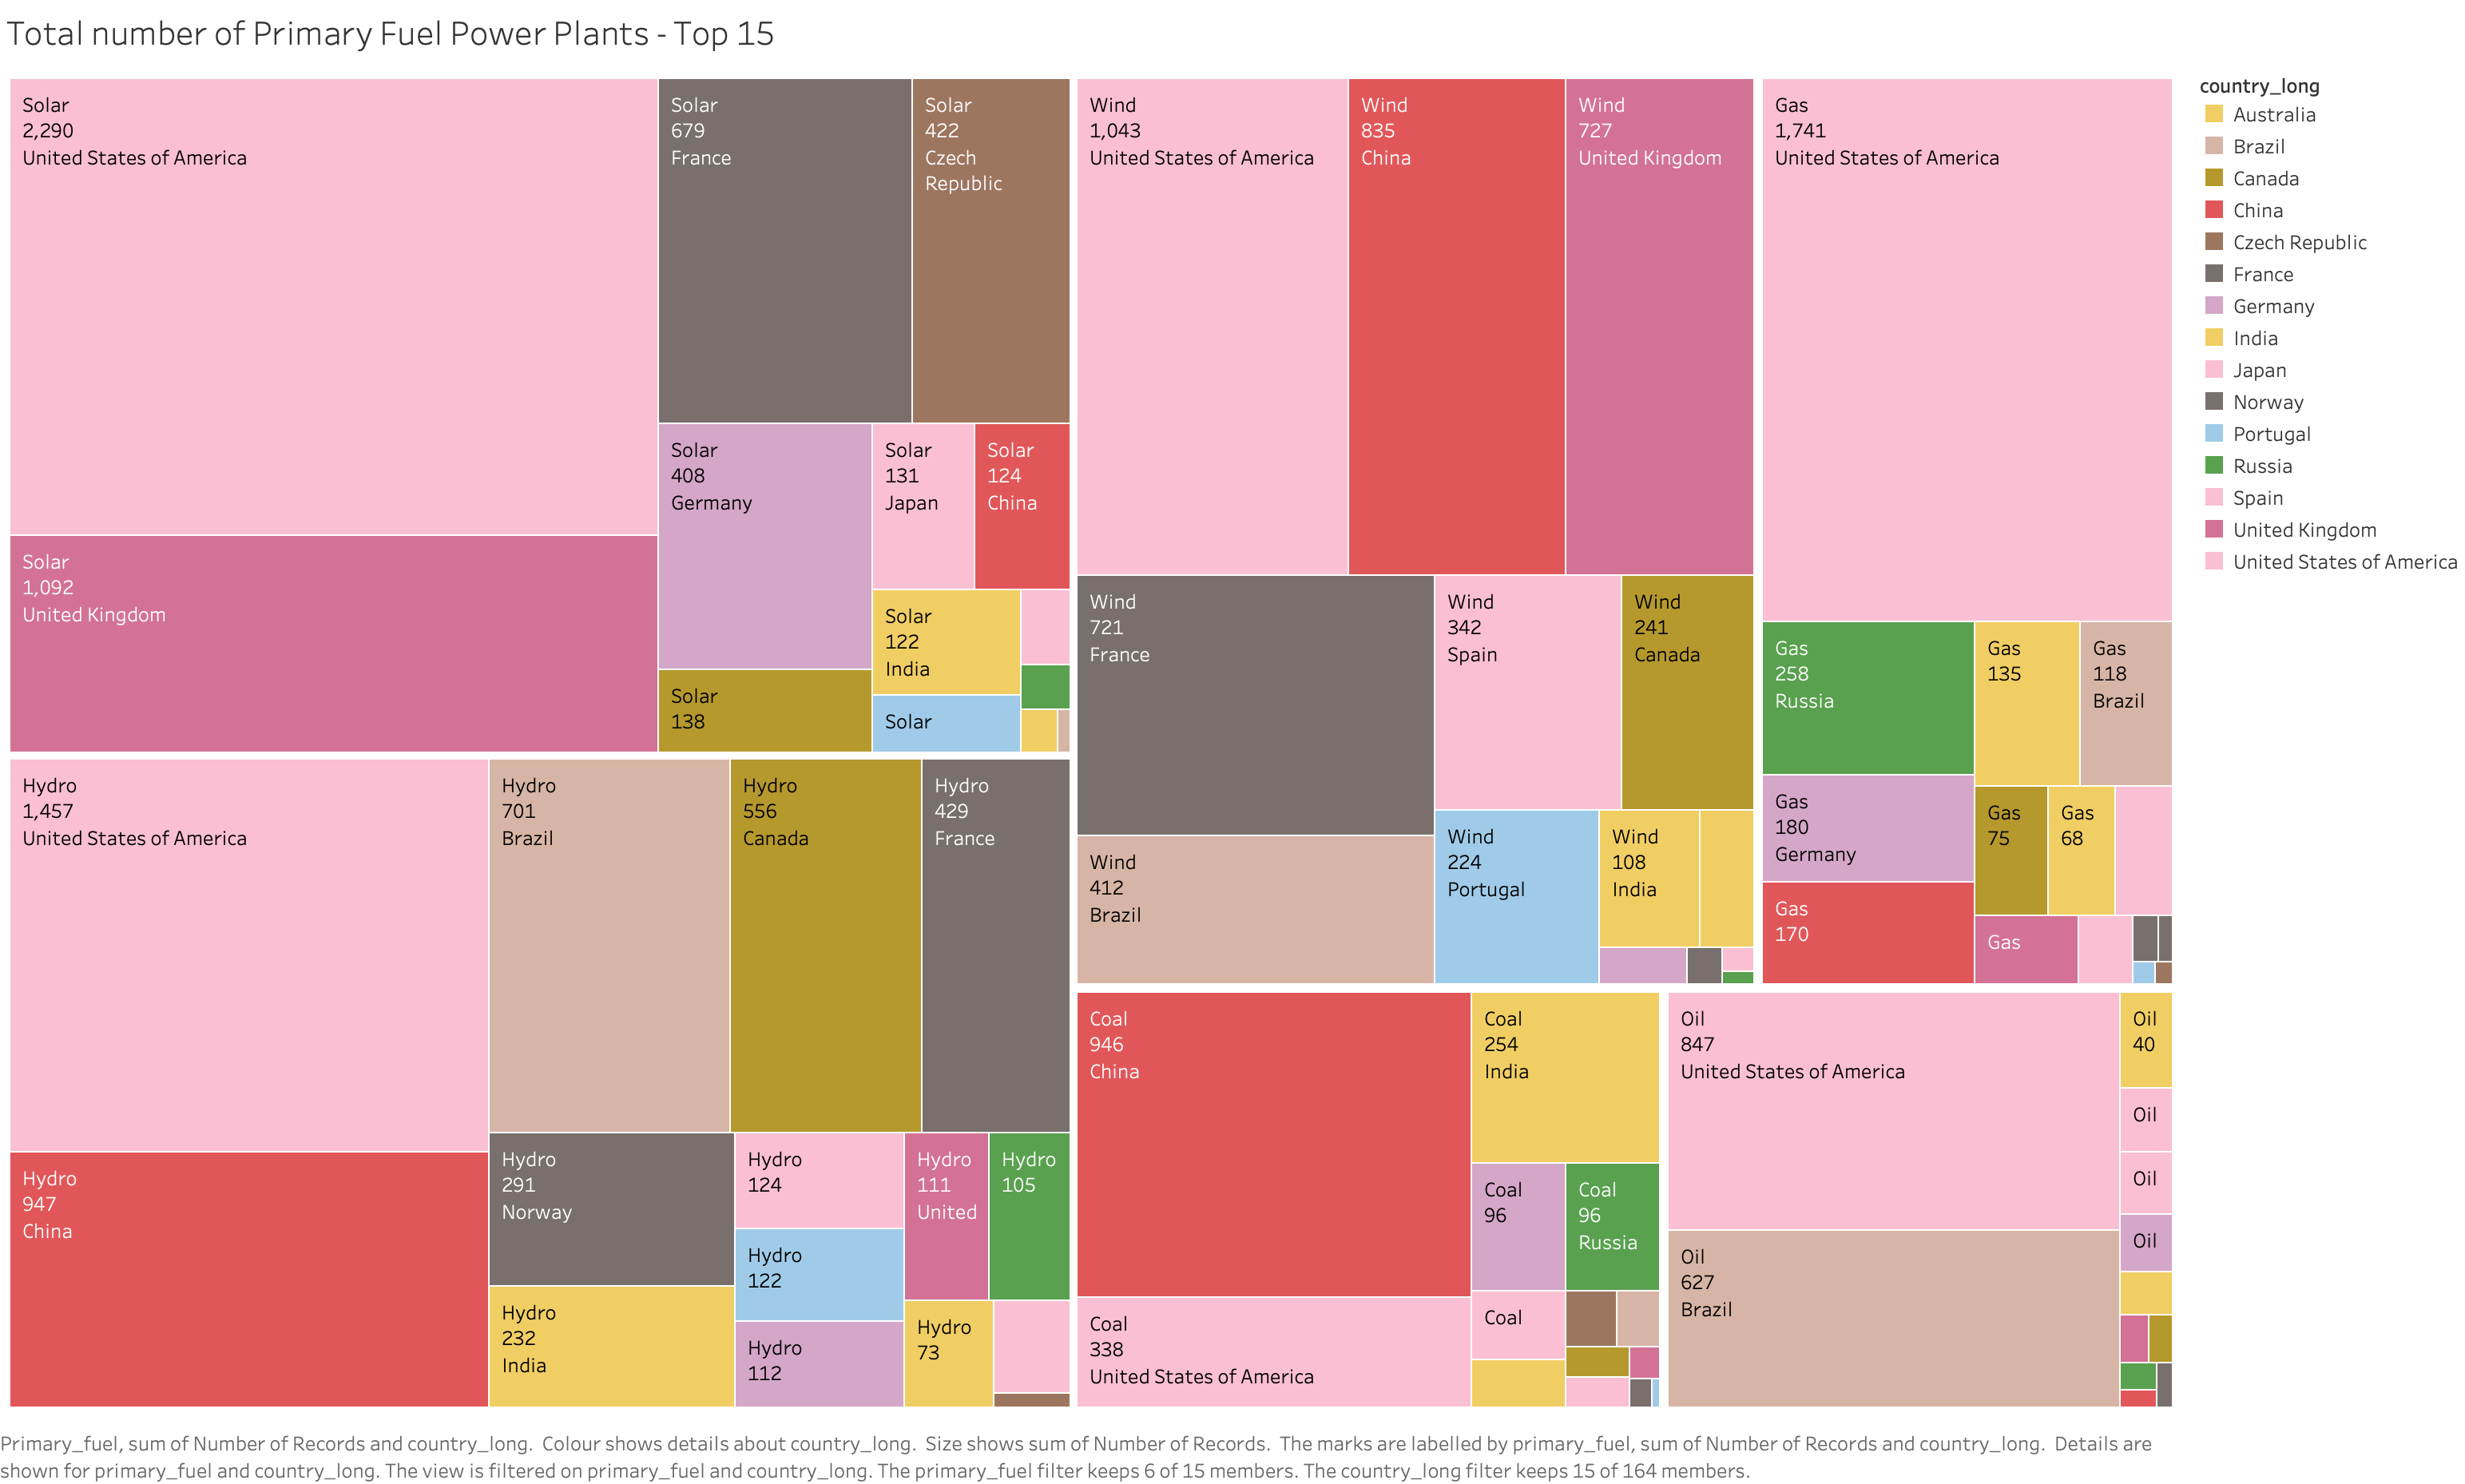
\includegraphics[width=15cm]{Numberofprifueltop15}

\begin{itemize}
\tightlist
\item
  \textbf{Name of Tool}: Tableau
\item
  \textbf{Country}: Australia, Brazil, Canada, China, Czech Republic, France, Germany, India, Japan, Norway, Portugal, Russia, Spain, United Kingdom, USA.
\item
  \textbf{Year}: 1896 - 2018.
\item
  \textbf{Data Preparation}: Top 6 values of the primary fuel was used as well as top 15 filter used for the counteries based on the sum of records.
\item
  \textbf{Color}: Colour has been assissiate to the different counteries.
\item
  \textbf{Hierarchy}: Each hierarchy is linked to the sum of the power plants based on their primary fuel. For example: Solar. 
\item
  What leaf node size is mapped to? This is mapped to the amount of records each country has to the hierarchy primary fuel type.
\item
  How are the leaf nodes laid out or positioned? The leaf nodes are laid out on top of the main hierarchy, each in the shape of a square, with the size of th esquare referencing the size of the record. For example, the bigger the square/rectangle the bigger that record is.
\item
  What are internal nodes mapped to?
\item
  What is internal node size mapped to?
\item
  Which treemap node layout algorithm is used?
  Tableau built in algorithm.
\end{itemize}
